\addcontentsline{toc}{chapter}{LAMPIRAN}
\chapter*{LAMPIRAN}

\section*{Lampiran 1. \normalfont{Peralatan penelitian}}
\label{Lampiran 1}
\begin{longtable}{c >{\centering\arraybackslash}m{4cm} m{8cm}}
  \toprule
  \textbf{No.} & \textbf{Alat dan Bahan} & \textbf{Fungsi} \\
  \midrule
  \endfirsthead

  \toprule
  \textbf{No.} & \textbf{Alat dan Bahan} & \textbf{Fungsi} \\
  \midrule
  \endhead

  \bottomrule
  \endfoot
  1 &
  \begin{tabular}[c]{@{}c@{}}
    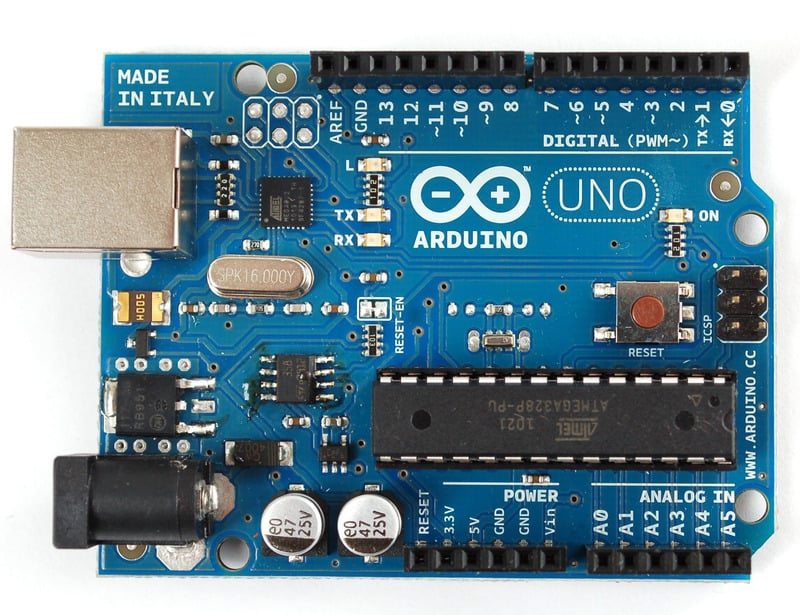
\includegraphics[width=2cm]{gambar/lampiran/arduino.jpg} \\
    Arduino Uno
  \end{tabular}
  & \vspace*{0.5cm} Berfungsi sebagai mikrokontroler utama yang
  mengendalikan motor servo pada lengan robot dan menerima sinyal
  dari sensor. \\
  2 &
  \begin{tabular}[c]{@{}c@{}}
    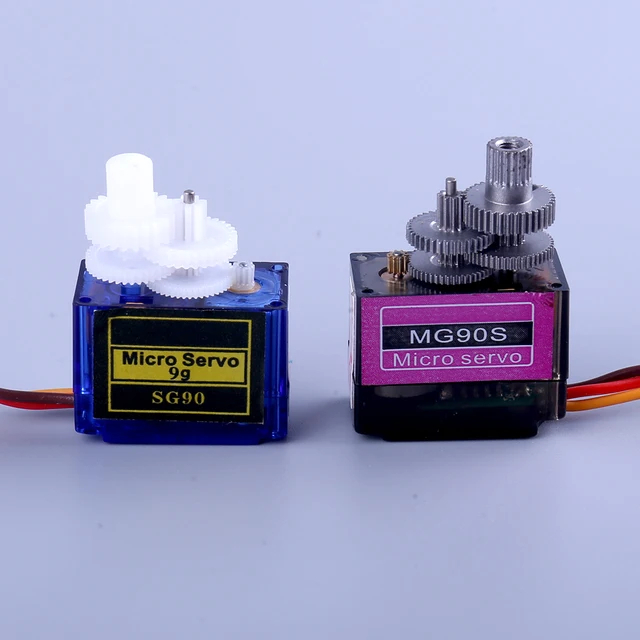
\includegraphics[width=2cm]{gambar/lampiran/servo.jpg} \\
    Motor \textit{servo}
  \end{tabular}
  & \vspace*{0.5cm} digunakan sebagai aktuator untuk menggerakkan
  bagian-bagian lengan robot sesuai perintah dari arduino. \\
  3 &
  \begin{tabular}[c]{@{}c@{}}
    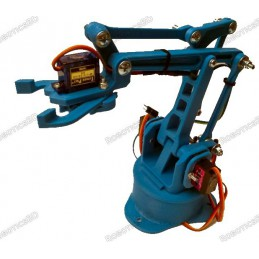
\includegraphics[width=2cm]{gambar/lampiran/robot.jpg} \\
    Lengan Robot
  \end{tabular}
  & \vspace*{0.5cm} struktur mekanik tempat pemasangan motor servo
  dan berperan sebagai sistem penggerak robotik. \\
  4 &
  \begin{tabular}[c]{@{}c@{}}
    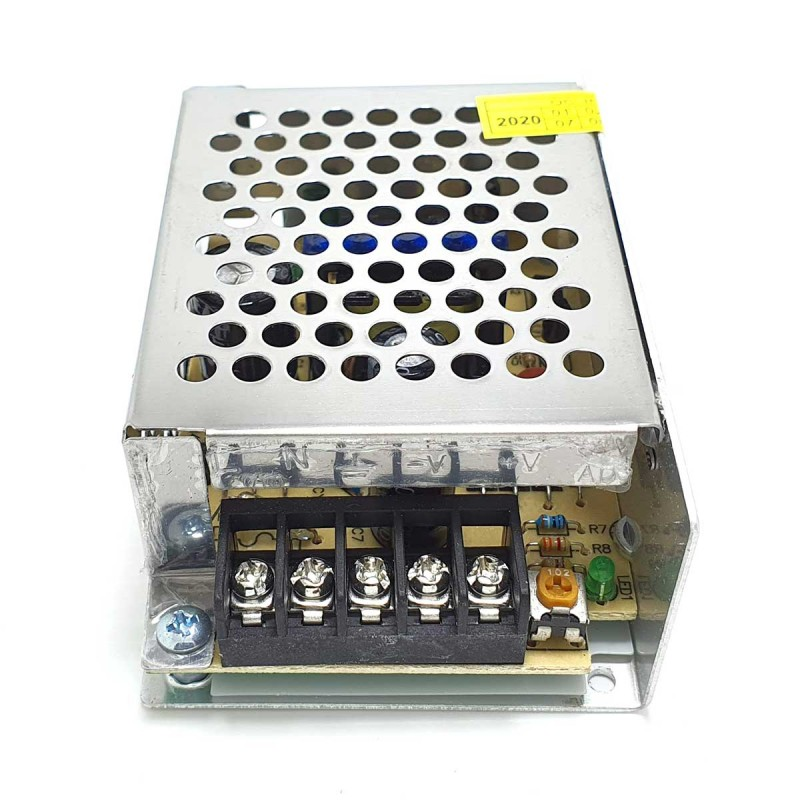
\includegraphics[width=2cm]{gambar/lampiran/psu.jpg} \\
    \textit{Power Supply} 5V
  \end{tabular}
  & \vspace*{0.5cm} Berfungsi menyediakan tegangan stabil untuk
  pengoperasian motor \textit{servo}. \\
  5 &
  \begin{tabular}[c]{@{}c@{}}
    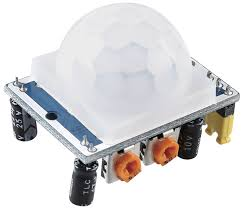
\includegraphics[width=2cm]{gambar/lampiran/pir.jpg} \\
    Sensor PIR
  \end{tabular}
  & \vspace*{0.5cm} Digunakan untuk mendeteksi pergerakan dan
  membantu menghitung jumlah kontainer cacat dan maupun tidak cacat
  yang melintas. \\
  6 &
  \begin{tabular}[c]{@{}c@{}}
    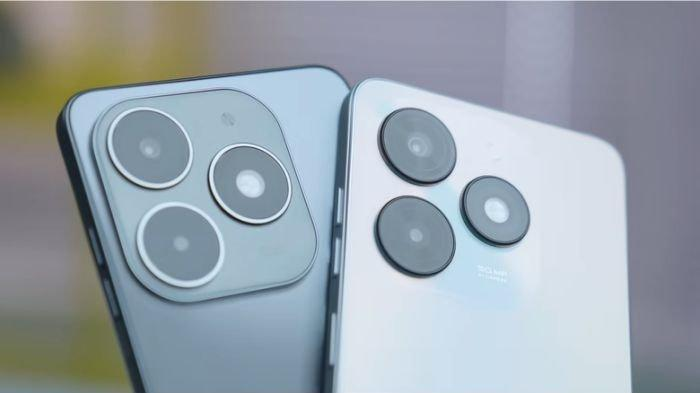
\includegraphics[width=2cm]{gambar/lampiran/kamera.jpg} \\
    Kamera
  \end{tabular}
  & \vspace*{0.5cm} Digunakan untuk mengambil citra kontainer kimia,
  yang akan diproses oleh model deteksi objek (YOLO) dan deteksi
  kecacatan (\textit{autoencoder}). \\
  7 &
  \begin{tabular}[c]{@{}c@{}}
    
\includegraphics[width=2cm]{gambar/lampiran/laptop.jpg} \\
    Laptop/Komputer
  \end{tabular}
  & \vspace*{0.5cm} Digunakan untuk memuat program ke Arduino Uno,
  serta menjalankan model deteksi objek berbasis YOLO dan
  \textit{autoencoder} untuk analisis visual. \\
  8 &
  \begin{tabular}[c]{@{}c@{}}
    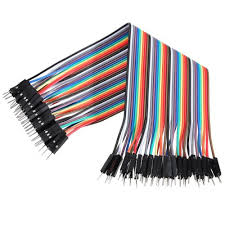
\includegraphics[width=2cm]{gambar/lampiran/jumper.jpg} \\
    Kabel \textit{Jumper}
  \end{tabular}
  & \vspace*{0.5cm} berfungsi menghubungkan berbagai komponen
  elektronik seperti sensor dan aktuator ke papan rangkaian dan Arduino. \\
  9 &
  \begin{tabular}[c]{@{}c@{}}
    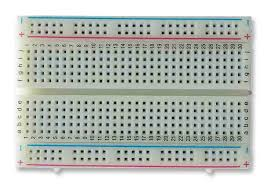
\includegraphics[width=2cm]{gambar/lampiran/breadboard.jpg} \\
    Papan Rangkaian
  \end{tabular}
  & \vspace*{0.5cm}berfungsi untuk menyediakan jalur koneksi antar komponen. \\
  \bottomrule
\end{longtable}

\vspace*{1em}

\section*{Lampiran 2. \normalfont{Hasil Perhitungan MSE untuk Beberapa Sampel}}
\label{Lampiran 2}
{\small
  \noindent\textbf{Catatan:} Perbedaan kecil pada hasil MSE hasil dan
  lampiran disebabkan oleh sifat probabilistik VAE. Setiap prediksi
  melibatkan sampling acak di ruang laten, sehingga hasil bisa
  sedikit bervariasi namun tidak signifikan.
}
\begin{enumerate}
  \item Normal
    \begin{align*}
      MSE &= \frac{1}{n} \sum_{i=1}^{n} (x_i - \hat{x}_i)^2 \\
      &= \frac{1}{128 \times 128 \times 3} (318,6943) \\
      &= \frac{318,6943}{49152} \\
      &= 0,006483
    \end{align*}
  \item Cacat
    \begin{align*}
      &= \frac{1}{128 \times 128 \times 3} (399,1252) \\
      &= \frac{399,1252}{49152} \\
      &= 0,008120
    \end{align*}
  \item Normal
    \begin{align*}
      &= \frac{1}{128 \times 128 \times 3} (332,1946) \\
      &= \frac{332,1946}{49152} \\
      &= 0,006758
    \end{align*}
  \item Normal
    \begin{align*}
      &= \frac{1}{128 \times 128 \times 3} (337,3314) \\
      &= \frac{337.3314}{49152} \\
      &= 0,006863
    \end{align*}
  \item Normal
    \begin{align*}
      &= \frac{1}{128 \times 128 \times 3} (330,1660) \\
      &= \frac{330,1660}{49152} \\
      &= 0,006717
    \end{align*}
  \item Cacat
    \begin{align*}
      &= \frac{1}{128 \times 128 \times 3} (369,0964) \\
      &= \frac{369,0964}{49152} \\
      &= 0,007509
    \end{align*}
  \item Cacat
    \begin{align*}
      &= \frac{1}{128 \times 128 \times 3} (355,1892) \\
      &= \frac{355,1892}{49152} \\
      &= 0,007226
    \end{align*}
  \item Cacat
    \begin{align*}
      &= \frac{1}{128 \times 128 \times 3} (355,7173) \\
      &= \frac{355,7173}{49152} \\
      &= 0,007237
    \end{align*}
  \item Normal
    \begin{align*}
      &= \frac{1}{128 \times 128 \times 3} (328,9789) \\
      &= \frac{328,9789}{49152} \\
      &= 0,006693
    \end{align*}
  \item Cacat
    \begin{align*}
      &= \frac{1}{128 \times 128 \times 3} (377,8040) \\
      &= \frac{377,8040}{49152} \\
      &= 0,007686
    \end{align*}
\end{enumerate}

\vspace*{1em}

\section*{Lampiran 3. \normalfont{Program untuk latih model YOLO}}
\label{Lampiran 3}
\begin{lstlisting}[language=Python]
from ultralytics import YOLO
model = YOLO("yolo12n.pt")
results = model.train(data=config, epochs=50)
inference = model("frame_02318.jpg")
inference[0].show()
\end{lstlisting}

\newpage
\section*{Lampiran 4. \normalfont{Program untuk latih model
\textit{autoencoder}}}
\label{Lampiran 4}
\begin{lstlisting}[language=Python]
import os
import torch
import torch.nn as nn
import torch.nn.functional as F
import torch.optim as optim
from torch.utils.data import DataLoader
from torchvision import transforms, datasets
import torchvision.transforms as transforms
from PIL import Image
import matplotlib.pyplot as plt
import numpy as np

class CVAE(nn.Module):
    def __init__(self, latent_dim=128):
        super(CVAE, self).__init__()
        self.latent_dim = latent_dim
        self.encoder = nn.Sequential(
            nn.Conv2d(3, 32, kernel_size=4, stride=2, padding=1),
            nn.ReLU(),
            nn.Conv2d(32, 64, kernel_size=4, stride=2, padding=1),
            nn.ReLU(),
            nn.Conv2d(64, 128, kernel_size=4, stride=2, padding=1),
            nn.ReLU(),
            nn.Conv2d(128, 256, kernel_size=4, stride=2, padding=1),
            nn.ReLU(),
            nn.Conv2d(256, 512, kernel_size=4, stride=2, padding=1),
            nn.ReLU()
        )
        self.fc_mu = nn.Linear(512 * 4 * 4, latent_dim)
        self.fc_logvar = nn.Linear(512 * 4 * 4, latent_dim)
        self.decoder_input = nn.Linear(latent_dim, 512 * 4 * 4)
        self.decoder = nn.Sequential(
            nn.ConvTranspose2d(512, 256, kernel_size=4, stride=2, padding=1),
            nn.ReLU(),
            nn.ConvTranspose2d(256, 128, kernel_size=4, stride=2, padding=1),
            nn.ReLU(),
            nn.ConvTranspose2d(128, 64, kernel_size=4, stride=2, padding=1),
            nn.ReLU(),
            nn.ConvTranspose2d(64, 32, kernel_size=4, stride=2, padding=1),
            nn.ReLU(),
            nn.ConvTranspose2d(32, 3, kernel_size=4, stride=2, padding=1),
            nn.Sigmoid()
        )

    def reparameterisasi(self, mu, logvar):
        """reparameterisasi agar ruang latent serupa dengan distribusi gaussian."""
        std = torch.exp(0.5 * logvar)
        eps = torch.randn_like(std)
        return mu + eps * std

    def forward(self, x):
        enc = self.encoder(x)
        enc = enc.view(x.size(0), -1)
        mu = self.fc_mu(enc)
        logvar = self.fc_logvar(enc)
        z = self.reparameterisasi(mu, logvar)
        dec_input = self.decoder_input(z)
        dec_input = dec_input.view(x.size(0), 512, 4, 4)
        reconstruction = self.decoder(dec_input)
        return reconstruction, mu, logvar

def fungsi_loss(recon_x, x, mu, logvar):
    """
    Menghitung VAE Loss yang terdiri dari MSE dan regularisasi
    """
    recon_loss = F.mse_loss(recon_x, x, reduction='sum')
    kl_loss = -0.5 * torch.sum(1 + logvar - mu.pow(2) - logvar.exp())
    return recon_loss + kl_loss

def train(model, dataloader, optimizer, device):
    model.train()
    train_loss = 0
    for batch_idx, (data, _) in enumerate(dataloader):
        data = data.to(device)
        optimizer.zero_grad()
        recon, mu, logvar = model(data)
        loss = fungsi_loss(recon, data, mu, logvar)
        loss.backward()
        train_loss += loss.item()
        optimizer.step()
        if batch_idx % 100 == 0:
            print(f'Batch {batch_idx}/{len(dataloader)} Loss: {loss.item()/len(data):.4f}')
    avg_loss = train_loss / len(dataloader.dataset)
    print(f'====> Average training loss: {avg_loss:.4f}')

def infer_anomaly_with_heatmap(image_path):
    """Inference gambar satuan dan tampilkan mse menggunakan heatmap."""

    image = Image.open(image_path).convert("RGB")
    image_tensor = transform(image).unsqueeze(0).to(device)

    with torch.no_grad():
        reconstructed, _, _ = model(image_tensor)

    anomaly_map = torch.abs(image_tensor - reconstructed).mean(dim=1, keepdim=True)

    anomaly_map = anomaly_map.squeeze().cpu().numpy()
    anomaly_map = (anomaly_map - anomaly_map.min()) / (anomaly_map.max() - anomaly_map.min())

    orig_np = image_tensor.squeeze(0).permute(1, 2, 0).cpu().numpy()
    recon_np = reconstructed.squeeze(0).permute(1, 2, 0).cpu().numpy()

    fig, axs = plt.subplots(1, 3, figsize=(12, 4))

    axs[0].imshow(orig_np)
    axs[0].set_title("Original Image")
    axs[0].axis("off")

    axs[1].imshow(recon_np)
    axs[1].set_title("Reconstructed Image")
    axs[1].axis("off")

    axs[2].imshow(orig_np)
    axs[2].imshow(anomaly_map, cmap='jet', alpha=0.5)
    axs[2].set_title("Anomaly Heatmap")
    axs[2].axis("off")

    plt.show()

    mse_loss = torch.mean((reconstructed - image_tensor) ** 2).item()
    print(f"Reconstruction Error (MSE): {mse_loss:.6f}")

    threshold = 0.007183
    is_anomalous = mse_loss > threshold
    print(f"Anomaly Detected: {is_anomalous}")

    return mse_loss, is_anomalous

if __name__ == "__main__":
    device = torch.device("cuda" if torch.cuda.is_available() else "cpu")

    transform = transforms.Compose([
        transforms.Resize((128, 128)),
        transforms.ToTensor(),
    ])

    train_dir = "data_ae/train"

    train_dataset = datasets.ImageFolder(train_dir, transform=transform)

    train_loader = DataLoader(train_dataset, batch_size=64, shuffle=True, num_workers=4)

    model = CVAE(latent_dim=128).to(device)
    optimizer = optim.Adam(model.parameters(), lr=1e-3)
    epochs = 50

    for epoch in range(1, epochs + 1):
        print(f"Epoch {epoch}/{epochs}")
        train(model, train_loader, optimizer, device)

\end{lstlisting}

\newpage
\section*{Lampiran 5. \normalfont{Program kombinasi YOLO dan
\textit{autoencoder}}}
\label{Lampiran 5}
\begin{lstlisting}[language=Python]
import cv2
import torch
import torch.nn as nn
import torchvision.transforms as transforms
from PIL import Image
from ultralytics import YOLO
import time
import collections
import serial
import os
from datetime import datetime
import matplotlib.pyplot as plt

class CVAE(nn.Module):
    def __init__(self, latent_dim=128):
        super(CVAE, self).__init__()
        self.latent_dim = latent_dim
        self.encoder = nn.Sequential(
            nn.Conv2d(3, 32, kernel_size=4, stride=2, padding=1),
            nn.ReLU(),
            nn.Conv2d(32, 64, kernel_size=4, stride=2, padding=1),
            nn.ReLU(),
            nn.Conv2d(64, 128, kernel_size=4, stride=2, padding=1),
            nn.ReLU(),
            nn.Conv2d(128, 256, kernel_size=4, stride=2, padding=1),
            nn.ReLU(),
            nn.Conv2d(256, 512, kernel_size=4, stride=2, padding=1),
            nn.ReLU(),
        )
        self.fc_mu = nn.Linear(512 * 4 * 4, latent_dim)
        self.fc_logvar = nn.Linear(512 * 4 * 4, latent_dim)
        self.decoder_input = nn.Linear(latent_dim, 512 * 4 * 4)
        self.decoder = nn.Sequential(
            nn.ConvTranspose2d(512, 256, kernel_size=4, stride=2, padding=1),
            nn.ReLU(),
            nn.ConvTranspose2d(256, 128, kernel_size=4, stride=2, padding=1),
            nn.ReLU(),
            nn.ConvTranspose2d(128, 64, kernel_size=4, stride=2, padding=1),
            nn.ReLU(),
            nn.ConvTranspose2d(64, 32, kernel_size=4, stride=2, padding=1),
            nn.ReLU(),
            nn.ConvTranspose2d(32, 3, kernel_size=4, stride=2, padding=1),
            nn.Sigmoid(),
        )

    def reparameterisasi(self, mu, logvar):
        """reparameterisasi agar ruang latent serupa dengan distribusi gaussian."""
        std = torch.exp(0.5 * logvar)
        eps = torch.randn_like(std)
        return mu + eps * std

    def forward(self, x):
        enc = self.encoder(x)
        enc = enc.view(x.size(0), -1)
        mu = self.fc_mu(enc)
        logvar = self.fc_logvar(enc)
        z = self.reparameterisasi(mu, logvar)
        dec_input = self.decoder_input(z)
        dec_input = dec_input.view(x.size(0), 512, 4, 4)
        reconstruction = self.decoder(dec_input)
        return reconstruction, mu, logvar

def get_centroid(x1, y1, x2, y2):
    return ((x1 + x2) // 2, (y1 + y2) // 2)

def check_anomaly(crop_img):
    image = Image.fromarray(cv2.cvtColor(crop_img, cv2.COLOR_BGR2RGB))
    image_tensor = transform(image).unsqueeze(0).to(device)
    with torch.no_grad():
        reconstructed, _, _ = ae_model(image_tensor)
    mse_loss = torch.mean((reconstructed - image_tensor) ** 2).item()
    return mse_loss

def save_anomaly_heatmap(image_tensor, reconstructed, loss_value, obj_id):
    anomaly_map = torch.abs(image_tensor - reconstructed).mean(dim=1, keepdim=True)
    anomaly_map = anomaly_map.squeeze().cpu().numpy()
    anomaly_map = (anomaly_map - anomaly_map.min()) / (
        anomaly_map.max() - anomaly_map.min() + 1e-8
    )

    orig_np = image_tensor.squeeze(0).permute(1, 2, 0).cpu().numpy()
    recon_np = reconstructed.squeeze(0).permute(1, 2, 0).cpu().numpy()

    fig, axs = plt.subplots(1, 3, figsize=(12, 4))

    axs[0].imshow(orig_np)
    axs[0].set_title("Original Image")
    axs[0].axis("off")

    axs[1].imshow(recon_np)
    axs[1].set_title("Reconstructed Image")
    axs[1].axis("off")

    axs[2].imshow(orig_np)
    axs[2].imshow(anomaly_map, cmap="jet", alpha=0.5)
    axs[2].set_title(f"Anomaly Heatmap\nLoss: {loss_value:.6f}")
    axs[2].axis("off")

    os.makedirs("output", exist_ok=True)
    timestamp = datetime.now().strftime("%Y%m%d_%H%M%S")
    filename = f"output/heatmap_{obj_id}_{timestamp}.png"
    plt.savefig(filename)
    plt.close(fig)

    print(f"[Saved] Heatmap image saved to {filename}")

TRANSFORM = transforms.Compose([transforms.Resize((128, 128)), transforms.ToTensor()])
DEVICE = torch.device("cuda" if torch.cuda.is_available() else "cpu")
AE_MODEL_PATH = "ae.pth"
YOLO_MODEL_PATH = "./runs/detect/train/weights/best.pt"
CONFIDENCE_THRESHOLD = 0.90
LOSS_BATCH_SIZE = 20
DELAY_SECONDS = 0.005
OBJECT_WARMUP_FRAMES = 5
CENTROID_TOLERANCE = 30
SPIKE_FILTER_THRESHOLD = 0.0099
SERIAL_PORT = "/dev/ttyACM0"
BAUD_RATE = 9600
DEFECT_THRESHOLD = 0.007183

print("Loading models...")
device = DEVICE
transform = TRANSFORM
ae_model = CVAE(latent_dim=128).to(device)
ae_model.load_state_dict(torch.load(AE_MODEL_PATH, map_location=device))
ae_model.eval()
yolo_model = YOLO(YOLO_MODEL_PATH)
print(f"Models loaded successfully on {device}.")

print("Initializing camera...")
cap = cv2.VideoCapture(0)
if not cap.isOpened():
    print("Error: Cannot open camera")
    exit()
print("Camera initialized.")

arduino = None
try:
    print(f"Connecting to Arduino on {SERIAL_PORT}...")
    arduino = serial.Serial(SERIAL_PORT, BAUD_RATE, timeout=1)
    time.sleep(2)
    print("Arduino connected.")
except serial.SerialException as e:
    print(f"WARNING: Could not connect to Arduino. {e}")
    print("--> Running in SIMULATION MODE. No data will be sent.")

object_history = collections.defaultdict(dict)

print("\nStarting monitoring... Press Ctrl+C to exit.")
try:
    while True:
        ret, frame = cap.read()
        if not ret:
            print("Failed to grab frame. Exiting.")
            break

        results = yolo_model(frame, verbose=False)[0]
        current_time = time.time()

        for box in results.boxes:
            if box.conf[0] < CONFIDENCE_THRESHOLD:
                continue

            x1, y1, x2, y2 = map(int, box.xyxy[0])
            crop = frame[y1:y2, x1:x2]
            centroid = get_centroid(x1, y1, x2, y2)

            for obj_id in list(object_history.keys()):
                if (
                    current_time - object_history[obj_id].get("last_seen", current_time)
                    > 2
                ):
                    print(f"[Cleanup] Removing stale object ID {obj_id}")
                    del object_history[obj_id]

            matched_id = None
            for obj_id, data in object_history.items():
                prev_centroid = data.get("last_centroid")
                if (
                    prev_centroid
                    and abs(prev_centroid[0] - centroid[0]) < CENTROID_TOLERANCE
                    and abs(prev_centroid[1] - centroid[1]) < CENTROID_TOLERANCE
                ):
                    data["seen_frames"] += 1
                    data["last_centroid"] = centroid
                    data["last_seen"] = current_time
                    matched_id = obj_id
                    break

            if matched_id is None:
                matched_id = len(object_history)
                object_history[matched_id] = {
                    "seen_frames": 1,
                    "last_centroid": centroid,
                    "valid_losses": [],
                    "first_sent": False,
                    "last_seen": current_time,
                }
                print(f"[New Object] Assigned ID {matched_id}")

            current_obj = object_history[matched_id]

            if current_obj["seen_frames"] <= OBJECT_WARMUP_FRAMES:
                print(
                    f"[Warmup] Skipping object {matched_id}, frame {current_obj['seen_frames']}"
                )
                continue

            anomaly_score = check_anomaly(crop)

            if anomaly_score > SPIKE_FILTER_THRESHOLD:
                print(f"[Spike Filter] Score {anomaly_score:.6f} too high, ignored.")
                current_obj["valid_losses"].clear()
                continue

            current_obj["valid_losses"].append(anomaly_score)

            if len(current_obj["valid_losses"]) >= LOSS_BATCH_SIZE:
                avg_error = sum(current_obj["valid_losses"]) / len(
                    current_obj["valid_losses"]
                )

                if not current_obj["first_sent"]:
                    print(
                        f"[Skip First Send] Skipping first Arduino send for object {matched_id}"
                    )
                    current_obj["first_sent"] = True
                    current_obj["valid_losses"].clear()
                    continue

                image_tensor = (
                    transform(Image.fromarray(cv2.cvtColor(crop, cv2.COLOR_BGR2RGB)))
                    .unsqueeze(0)
                    .to(device)
                )
                with torch.no_grad():
                    reconstructed, _, _ = ae_model(image_tensor)

                save_anomaly_heatmap(image_tensor, reconstructed, avg_error, matched_id)

                print(f"[*] Object {matched_id} final avg loss: {avg_error:.6f}")
                label = "DEFECT" if avg_error > DEFECT_THRESHOLD else "OK"
                msg = f"{label},{avg_error:.6f}\n"

                if arduino:
                    try:
                        print(f"--> Sending to Arduino: {msg.strip()}")
                        arduino.write(msg.encode())
                    except serial.SerialException as e:
                        print(f"ERROR: Arduino write failed: {e}. Disconnecting.")
                        arduino.close()
                        arduino = None
                else:
                    print(f"--> [SIMULATED] Arduino message: {msg.strip()}")

                current_obj["valid_losses"].clear()
            else:
                print(
                    f"[Collecting] Object {matched_id} sample {len(current_obj['valid_losses'])}/{LOSS_BATCH_SIZE}"
                )

        time.sleep(DELAY_SECONDS)

except KeyboardInterrupt:
    print("\nInterruption detected. Shutting down.")
finally:
    cap.release()
    print("Camera released.")
    if arduino and arduino.is_open:
        arduino.close()
        print("Arduino connection closed.")
    print("Exited gracefully.")
\end{lstlisting}

\newpage
\section*{Lampiran 6. \normalfont{Program lengan robot}}
\label{Lampiran 6}
\begin{lstlisting}[language=C++]
#include <Servo.h>
Servo servo2;
Servo servo3;
Servo servo4;

void write_servo(int from, int to, int delay_rotate, Servo &servo) {
  if (from < to) {
    for (int pos = from; pos <= to; pos++) {
      servo.write(pos);
      delay(delay_rotate);
    }
  } else {
    for (int pos = from; pos >= to; pos--) {
      servo.write(pos);
      delay(delay_rotate);
    }
  }
}

void setup() {
  servo2.attach(5);
  servo3.attach(6);
  servo4.attach(9);

  servo2.write(85);
  servo3.write(30);
  servo4.write(170);
  delay(2000);

  Serial.begin(9600);
}

void loop() {
  if (Serial.available()) {
    String msg = Serial.readStringUntil('\n');

    int sepIndex = msg.indexOf(',');
    if (sepIndex > 0) {
      String label = msg.substring(0, sepIndex);
      String errorStr = msg.substring(sepIndex + 1);
      float errorVal = errorStr.toFloat();

      if (label == "DEFECT" || label == "OK") {
        Serial.print(label);
        Serial.print(",");
        Serial.println(errorVal, 5);

        if (label == "DEFECT") {
          // KIRI
          write_servo(50, 120, 15, servo3);
          delay(2000);

          write_servo(170, 30, 5, servo4);
          delay(2000);

          write_servo(120, 50, 15, servo3);
          delay(2000);

          write_servo(85, 180, 30, servo2);
          delay(2000);

          write_servo(30, 170, 5, servo4);
          delay(2000);

          write_servo(180, 85, 30, servo2);
          delay(2000);

        } else if (label == "OK") {
          // KANAN
          write_servo(50, 120, 15, servo3);
          delay(2000);

          write_servo(170, 30, 5, servo4);
          delay(2000);

          write_servo(120, 50, 15, servo3);
          delay(2000);

          write_servo(85, 0, 30, servo2);
          delay(2000);

          write_servo(30, 170, 5, servo4);
          delay(2000);

          write_servo(0, 85, 30, servo2);
          delay(2000);
        }
      }
    }
  }
}
\end{lstlisting}

\vspace{1em}

\section*{Lampiran 7. \normalfont{Dokumentasi pergerakan lengan robot}}
\label{Lampiran 7}
\begin{figure}[H]
  \centering
  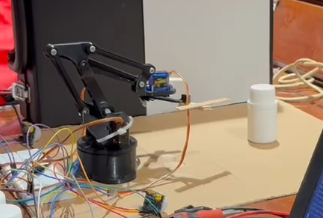
\includegraphics[width=0.8\textwidth]{gambar/lampiran/robot.png} \\
  Lengan robot menunggu hasil deteksi cacat
\end{figure}
\vspace{-1em}

\begin{figure}[H]
  \centering
  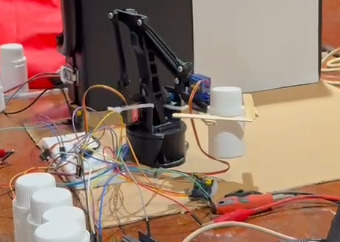
\includegraphics[width=0.8\textwidth]{gambar/robot_normal.jpeg} \\
  Lengan robot ketika meyortir kontainer normal
\end{figure}
\vspace{-1em}

\begin{figure}[H]
  \centering
  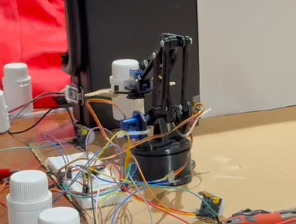
\includegraphics[width=0.8\textwidth]{gambar/robot_cacat.jpeg} \\
  Lengan robot ketika meyortir kontainer cacat
\end{figure}
\vspace{-1em}
